\subsection{Registradores e interface PCI}
\label{sec:impl.regs}

Nosso projeto define quatro registradores de \emph{software}, um
para cada porta de destino que deve ser bloqueada.  Estes
registradores de \emph{software} podem ser configurados
dinamicamente a partir do espaço de usuário.  Nós definimos os
registradores no arquivo XML de configuração do nosso projeto como
abaixo.

\begin{minted}{xml}
<!-- netfpga/projects/firewall/include/project.xml -->
<nf:name>firewall</nf:name>
   <nf:prefix>firewall</nf:prefix>
   <nf:location>udp</nf:location>
   <nf:description>Registers for minifirewall</nf:description>
   <nf:blocksize>128</nf:blocksize>
   <nf:registers>
      <nf:register>
         <nf:name>dport1</nf:name>
         <nf:description>Blocked port 1</nf:description>
         <nf:type>generic_software32</nf:type>
      </nf:register>
      ...
   </nf:registers>
\end{minted}

O programa \ssf{nf\_register\_gen} processa os arquivos XML de
configuração de todos os módulos de um projeto, gera um
identificador para cada módulo, calcula requisitos de armazenamento
para os registradores de cada módulo e gera endereços virtuais para
cada registrador.\footnotemark{}  O endereço virtual de um
registrador é composto do identificador do módulo onde foi declarado
e de seu deslocamento dentro do bloco de memória reservado aos
registradores do módulo.  Como nosso \emph{firewall} possui quatro
registradores de 32 bits para armazenar as portas TCP que estão
bloqueadas, definimos um bloco de registradores de 128 bits
(\ssf{blocksize} na configuração acima).  O tamanho do bloco de
registradores define a quantidade de bits necessárias para a parte
de deslocamento do endereço dos registradores.

\footnotetext{O arquivo XML com a configuração global do
\emph{firewall} está em
\url{netfpfa/projects/firewall/include/project.xml}.  Arquivos com a
configuração dos módulos estão no mesmo diretório.}

O \ssf{nf\_register\_gen} gera cabeçalhos Verilog, C, Python e Perl
contendo constantes que permitem endereçar os registradores em cada
uma destas linguagens.  Os arquivos de cabeçalho são necessários
para compilação de programas de usuário e sintetização do projeto em
\emph{hardware}.  O \ssf{nf\_register\_gen} pode ser executado com o
comando seguinte (os cabeçalhos são criados dentro da pasta
\ssf{netfpga/projects/firewall/lib/}):

\begin{minted}{bash}
netfpga/bin/nf_register_gen.pl --project firewall
\end{minted}

% \begin{table}[h]
% \centering
% \begin{tabular}{|l|l|l|}
% \hline
% \textbf{Macro}       & \textbf{Endereço Verilog} & \textbf{Endereço C} \\ \hline
% FIREWALL\_DPORT1 & 5'h0                      & 0x2000000           \\ \hline
% FIREWALL\_DPORT2 & 5'h1                      & 0x2000004           \\ \hline
% FIREWALL\_DPORT3 & 5'h2                      & 0x2000008           \\ \hline
% FIREWALL\_DPORT4 & 5'h3                      & 0x200000c           \\ \hline
% \end{tabular}
% \label{tab:impl.firewall.regs}
% \caption{Endereços virtuais em arquivos de cabeçalho C e Verilog dos registradores do firewall.}
% \end{table}

Os endereços virtuais de registradores em programas do usuário
possuem 28~bits e independem do tipo do registrador (contador,
\emph{software}, ou \emph{hardware}).  Como a NetFPGA interage com
sistemas operacionais de 32~bits, registradores maiores que 32 bits
são particionados em múltiplas palavras de 32~bits segundo o esquema
mostrado nas colunas ``64~bits'' e ``128~bits'' na
tabela~\ref{table:impl.regs.width}.

\begin{table}[h]
\centering
\begin{tabular}{llllll}
\multicolumn{2}{c}{\textbf{32 bits}} & \multicolumn{2}{c}{\textbf{64 bits}} & \multicolumn{2}{c}{\textbf{128 bits}} \\ \hline
\textbf{Macro}     & \textbf{Endereço} & \textbf{Macro}         & \textbf{Endereço} & \textbf{Macro}            & \textbf{Endereço} \\ \hline
\ssf{EX\_REG} & 0x2000004         & \ssf{EX\_REG\_LO} & 0x2000004         & \ssf{EX\_REG\_1\_LO} & 0x2000004   \\
                   &                   & \ssf{EX\_REG\_HI} & 0x2000008         & \ssf{EX\_REG\_1\_HI} & 0x2000008   \\
                   &                   &                        &                   & \ssf{EX\_REG\_2\_LO} & 0x200000c   \\
                   &                   &                        &                   & \ssf{EX\_REG\_2\_HI} & 0x2000010   \\
\end{tabular}
\caption{Exemplo do esquema de geração de nomes para registradores maiores que 32 bits.}
\label{table:impl.regs.width}
\end{table}

Registradores de \emph{software} podem ser escritos lidos e escritos
utilizando as funções \ssf{readReg} e \ssf{writeReg} definidas na
biblioteca de funções da NetFPGA (em \ssf{netfpga/lib}).  Por
exemplo, no nosso programa de configuração dinâmica das portas
bloqueadas, \ssf{nffw}, temos:

\begin{minted}{c}
   // netfpga/projects/firewall/sw/nffw.c
   writeReg(&nf2, FIREWALL_DPORT0_REG, dropped[0]);
   ...
   readReg(&nf2, FIREWALL_DPORT0_REG, &check[0]);
\end{minted}

A memória SRAM também pode ser acessada pela interface de
registradores.  A primeira palavra da memória SRAM é mapeada no
endereço virtual \ssf{SRAM\_BASE\_ADDR}, e outras palavras podem ser
acessadas indiretamente a partir de \ssf{SRAM\_BASE\_ADDR}.  O
seguinte exemplo zera as dez primeiras palavras da memória:

\begin{minted}{c}
   for(i = 0; i < 10; i++)
      unsigned offset = i*4; // 4 bytes per word
      writeReg(&nf2, SRAM_BASE_ADDR + offset, 0);
\end{minted}

Chamadas de função como \ssf{writeReg} enviam uma requisição de
escrita em registrador para a NetFPGA.  Essa requisição é recebida
pelo barramento PCI.  Para facilitar o processamento de requisições
de escrita e leitura dos registradores, podemos usar o módulo
\ssf{generic\_regs}.  O módulo \ssf{generic\_regs} é padrão no
pacote de \emph{software} da NetFPGA e é instanciado dentro dos
módulos que compõem o \emph{pipeline} de processamento.

Quando instanciamos o \ssf{generic\_regs}, definimos o número de
registradores e as linhas conectadas a cada registrador.  Definimos
também em qual módulo ele está sendo instanciado (parâmetro
\ssf{TAG}).  Esta informação permite à instância do
\ssf{generic\_regs} identificar os endereços dos registradores do
módulo e quais requisições de escrita e leitura em registradores
deve tratar.

\begin{verilogcode}
   generic_regs
   #(
      .TAG               (`FIREWALL_BLOCK_ADDR), // module ID
      .NUM_SOFTWARE_REGS (4),                    // number of sw regs
      ...
   ) module_regs (
      .reg_req_in       (reg_req_in),      // register bus input lines
      .reg_ack_in       (reg_ack_in),
      .reg_rd_wr_L_in   (reg_rd_wr_L_in),
      .reg_addr_in      (reg_addr_in),
      .reg_data_in      (reg_data_in),
      .reg_src_in       (reg_src_in),
      .reg_req_out      (reg_req_out),     // register bus output lines
      .reg_ack_out      (reg_ack_out),
      .reg_rd_wr_L_out  (reg_rd_wr_L_out),
      .reg_addr_out     (reg_addr_out),
      .reg_data_out     (reg_data_out),
      .reg_src_out      (reg_src_out),
      .counter_updates  (),                // register definitions
      .counter_decrement(),
      .software_regs    ({dport1, dport2, dport3, dport4}),
      .hardware_regs    (),
      ...
    );
\end{verilogcode}

As requisições de leitura e escrita em registradores recebidas pelo
barramento PCI são inseridas no barramento de registradores.  O
barramento de registradores é paralelo ao barramento de
encaminhamento.  Como no barramento de encaminhamento, cada
instância do módulo \ssf{generic\_regs} tem sinais de entrada
(sufixo \ssf{\_in}), para receber requisições do módulo anterior, e
de saída (sufixo \ssf{\_out}), para repassar as requisições ao
próximo módulo.  Ilustramos o barramento de registradores na
figura~\ref{fig:impl.regs.bus}.  A linha \ssf{req} indica se as
outras linhas carregam uma requisição válida.  As linhas \ssf{addr}
especificam o endereço virtual do registrador.  A linha
\ssf{rd\_wr\_L} indica se a requisição é de leitura ou escrita (com
lógica negativa, leitura quando ligado e escrita quando desligado) e
as linhas \ssf{data} contém o dado a ser escrito ou o dado lido.  A
linha \ssf{ack} indica se a requisição já foi tratada e as linhas
\ssf{src} indicam qual módulo tratou a requisição.

\begin{figure}
\centering
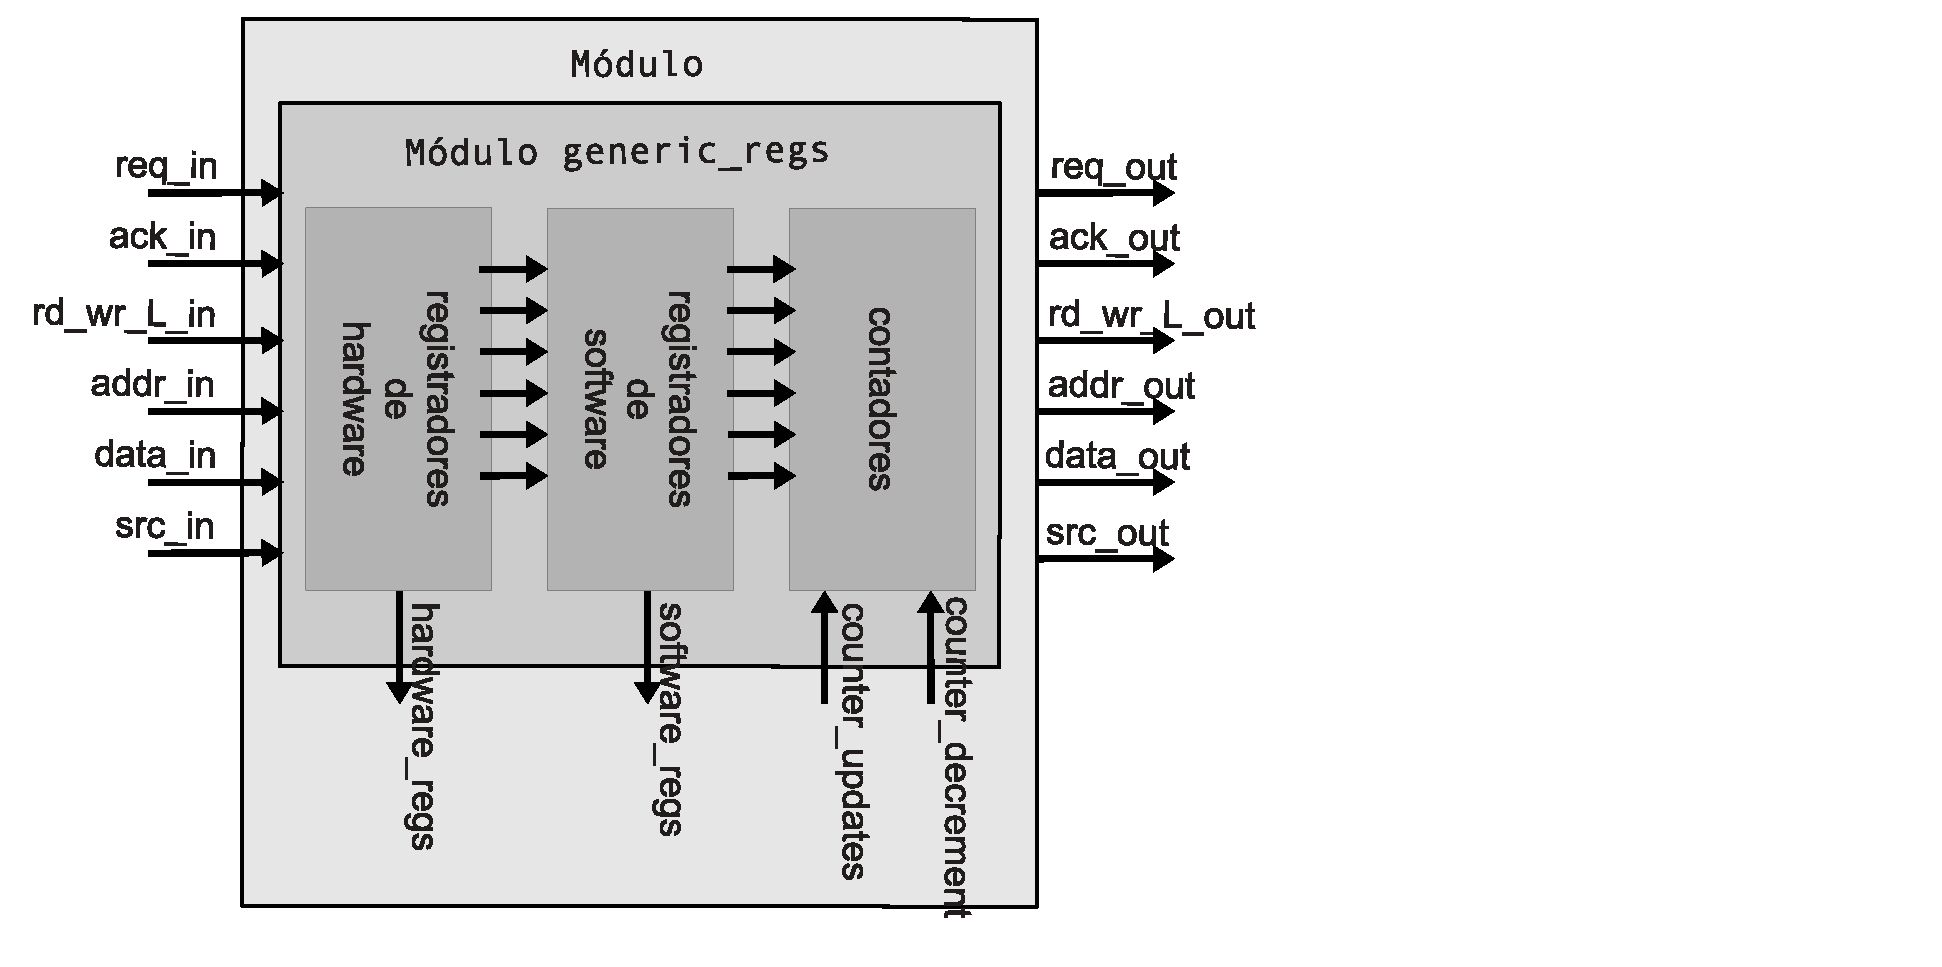
\includegraphics[scale=0.6,angle=0]{figures/modulos/genregister.eps}
\caption{Módulo \ssf{generic\_regs} e barramento de registradores.}
\label{fig:impl.regs.bus}
\end{figure}

O \ssf{nf\_register\_gen} gera blocos para armazenamento de
registradores automaticamente.  Para projetos com requisitos
específicos, é possível controlar o endereço base dos registradores
de cada módulo no arquivo XML de configuração do projeto.  Por
exemplo, para posicionar os registradores do nosso \emph{firewall}
no endereço \ssf{0x02000400} basta utilizar a configuração a seguir.

\begin{minted}{xml}
<!-- netfpga/projects/firewall/include/project.xml -->
<nf:memalloc layout="reference">
    <nf:group name="udp">
        <nf:instance name="firewall" base="0x02000400"/>
        ...
    </nf:group>
    ...
</nf:memalloc>
\end{minted}

Nosso \emph{firewall} lê as portas que devem ser filtradas da
memória SRAM (sexto estágio).  Esta decisão de projeto é didática,
para exemplificar a utilização da memória SRAM.  Num projeto real,
as portas poderiam ser lidas diretamente dos registradores
\ssf{dport0}, \ssf{dport1}, \ssf{dport2}, \ssf{dport3}.  Para que
possa ler as portas TCP bloqueadas da memória SRAM, nosso
\emph{firewall} precisa também gravar esta informação na memória.
Isto é realizado gravando os registradores na memória usando o
módulo \ssf{sram\_arbiter}.  Para detectar se as portas bloqueadas
foram modificadas, verificamos se o uma requisição de registrador
foi atendida (\ssf{reg\_ack\_out}) e se o endereço da requisição
pertence ao nosso módulo (\ssf{tag\_hit} e \ssf{addr\_good}).  Para
verificar se o endereço da requisição pertence ao nosso módulo,
utilizamos as constantes geradas pelo \ssf{nf\_register\_gen}.

\begin{verilogcode}
   always @(*) begin
      wr_data_next <= {dport3[15:0], dport2[15:0],
                       dport1[15:0], dport0[15:0]};
      wr_addr_next <= SRAM_PORTS_ADDR;
      if(tag_hit && addr_good && reg_ack_out)
         wr_req_next <= 1;
      else
         wr_req_next <= 0;
   end
   assign addr_block = reg_addr_out[`UDP_REG_ADDR_WIDTH-1:
                                    `FIREWALL_REG_ADDR_WIDTH];
   assign tag_hit = `FIREWALL_BLOCK_ADDR == addr_block;
   assign addr_good = reg_addr_out[`FIREWALL_REG_ADDR_WIDTH-1:0] >= 
    `FIREWALL_DPORT0 && reg_addr_out[`FIREWALL_REG_ADDR_WIDTH] <= 
    `FIREWALL_DPORT3;
\end{verilogcode}

As linhas \ssf{addr\_block} são construídas a partir do endereço da
requisição e contém o identificador do bloco de registradores (linha
10).  O identificador do bloco de registradores pode ser utilizado
para verificar se o registrador pertence ao nosso módulo (linha 12).
Por último, a linha \ssf{addr\_good} indica se o registrador escrito
é um dos registradores que armazena as portas TCP bloqueadas (linha
13).
